% ====================================================================
% === SUPERSEDED (reader-facing) by Docs/notes/03_multicore_siv.tex
%     (Vol-Fitter Technical Notes series). For the maintained,
%     comprehensive treatment with implementation + performance
%     appendices and code-generated figures, read that note.
% === RETAINED here as the equation-label citation source for code
%     docstrings, which reference this file by path and by its eq.
%     labels (e.g. "eq. q_logit", "note section 5.2").
% ====================================================================
\documentclass[11pt]{article}

\usepackage[margin=1in]{geometry}
\usepackage{amsmath,amssymb,amsfonts,mathtools}
\usepackage{booktabs}
\usepackage{array}
\usepackage{enumitem}
\usepackage{graphicx}
\usepackage{xcolor}
\usepackage{hyperref}
\usepackage{microtype}
\usepackage{listings}
\usepackage{caption}

\hypersetup{
  colorlinks=true,
  linkcolor=blue!50!black,
  citecolor=blue!50!black,
  urlcolor=blue!50!black
}

\lstset{
  basicstyle=\ttfamily\small,
  columns=fullflexible,
  breaklines=true,
  frame=single,
  xleftmargin=0.5em,
  xrightmargin=0.5em,
  language=Python,
  showstringspaces=false
}

\DeclareMathOperator{\sech}{sech}
\DeclareMathOperator{\argmin}{arg\,min}
\newcommand{\R}{\mathbb{R}}
\newcommand{\dd}{\mathrm{d}}
\newcommand{\eps}{\varepsilon}
\newcommand{\half}{\tfrac{1}{2}}
\newcommand{\bsigma}{\sigma_{\mathrm{BS}}}
\newcommand{\sigref}{\sigma_{\mathrm{ref}}}
\newcommand{\softplus}{\operatorname{softplus}}

\title{Generic Multi-Core Sigmoid Implied Variance\\
\large A sparse zero-wing kernel extension of SIV for WW-shaped volatility smiles}
\author{Technical note}
\date{13 June 2026}

\begin{document}
\maketitle

\begin{abstract}
The original Sigmoid-Implied Variance (SIV) slice models the second derivative of implied variance in normalized log-strike by a single sigmoid-derivative bell.  After two integrations this gives a log-cosh variance curve with smooth curvature, stable linear wings, and trader-readable controls for ATM level, ATM skew, ATM curvature, wing slopes, and minimum variance.  The single-core construction is deliberately parsimonious, but it is globally convex in implied variance when its structural kurtosis is positive.  It therefore cannot represent a genuine WW-shaped or dual-hat smile with two near-ATM shoulders and a central trough.

This note replaces the previous event-specific extension by a generic multi-core SIV model.  The model class is a base SIV slice plus a sparse sum of normalized zero-wing hat kernels.  Each hat is a second finite difference of the same log-cosh primitive already used by SIV.  The added kernels are $C^\infty$, have closed-form first and second derivatives, may carry positive or negative amplitudes, and vanish together with their slope and curvature in both tails.  Hence they add local shape flexibility without changing the original SIV wing slopes.  A three-core example shows how the model fits a synthetic WW-shaped smile using two positive shoulder hats and one negative central notch, while preserving Lee-compatible tails and passing a grid butterfly-arbitrage diagnostic.
\end{abstract}

\tableofcontents

\section{Purpose of the revision}

The model proposed here has no event switch, no event time, no event probability, and no event-specific term-structure layer.  Scheduled events may explain why a market smile has a dual-hat or WW geometry, but the parameterization itself should not depend on that interpretation.  The model class is simply
\begin{equation}
  \boxed{
  v_{R}(z)
  = v_{\mathrm{base}}(z;\theta)
    + \sum_{r=1}^{R}\alpha_r B_{c_r,h_r,\kappa_r}(z),
  \qquad R\in\{0,1,2,3,\ldots\}.
  }
  \label{eq:main-model}
\end{equation}
Here $v$ denotes annualized Black-Scholes implied variance and
\begin{equation}
  z=\frac{k}{\sigref\sqrt{T}},\qquad k=\log(K/F),
  \label{eq:z-def}
\end{equation}
where $F$ is the forward and $T$ is maturity.  The coordinate $z$ is the dimensionless log-strike coordinate used in the original SIV documentation \cite{sivdoc}.  The base slice $v_{\mathrm{base}}$ is the original one-core SIV, or any already-approved SIV slice.  The functions $B_{c,h,\kappa}$ are normalized local hats.  Positive amplitudes $\alpha_r$ add local variance humps; negative amplitudes add local notches.

The important distinction is the following.
\begin{itemize}[leftmargin=2em]
  \item A \emph{positive} multi-core model is still globally convex in implied variance and cannot generate a true WW smile.
  \item A \emph{signed raw} multi-core model can generate WW shapes, but unconstrained raw signed cores generally move the wings.
  \item A \emph{signed zero-wing} multi-core model gives the desired local flexibility while leaving the SIV wing map untouched.
\end{itemize}
The rest of the note makes this precise.

\section{Baseline: one-core SIV}

The SIV slice starts by prescribing the second derivative of implied variance in $z$-space.  In structural notation,
\begin{equation}
  v''(z)
  =K_0\sech^2\!\left(\frac{\kappa_i(z-z_0)}{2}\right),
  \qquad
  \kappa_i=
  \begin{cases}
    \kappa_P, & z<z_0,\\
    \kappa_C, & z\ge z_0.
  \end{cases}
  \label{eq:siv-convexity}
\end{equation}
The integrations are closed form:
\begin{align}
  v'(z)
  &= S_0+\frac{2K_0}{\kappa_i}
  \tanh\!\left(\frac{\kappa_i(z-z_0)}{2}\right),
  \label{eq:siv-slope}\\
  v(z)
  &= V_0+S_0(z-z_0)
  +\frac{4K_0}{\kappa_i^2}
  \log\cosh\!\left(\frac{\kappa_i(z-z_0)}{2}\right).
  \label{eq:siv-variance}
\end{align}
The trader wing slopes determine the transition speeds through
\begin{equation}
  \kappa_P=\frac{2K_0}{S_0+W_P},
  \qquad
  \kappa_C=\frac{2K_0}{W_C-S_0},
  \label{eq:siv-wing-map}
\end{equation}
which implies
\begin{equation}
  \lim_{z\to-\infty}v'(z)=-W_P,
  \qquad
  \lim_{z\to+\infty}v'(z)=W_C.
  \label{eq:siv-wing-limits}
\end{equation}
Thus the one-core SIV slice is built around six trader inputs,
\begin{equation}
  \big(v(0),\;v'(0),\;v''(0),\;W_P,\;W_C,\;v_{\min}\big),
  \label{eq:siv-trader-params}
\end{equation}
which are mapped to the structural engine parameters $(V_0,S_0,K_0,z_0,\kappa_P,\kappa_C)$ \cite{sivdoc}.

The log-cosh formula should be evaluated using the stable identity
\begin{equation}
  \log\cosh x = |x|-\log 2+O(e^{-2|x|})
  \qquad (|x|\to\infty),
  \label{eq:safe-logcosh}
\end{equation}
which avoids overflow for large $|x|$.

\section{Why more positive cores are not enough}
\label{sec:positive-cores}

The one-core SIV slice with $K_0>0$ satisfies $v''(z)\ge0$ for all $z$.  Hence $v'$ is monotone and $v$ has at most one stationary point.  Since $\bsigma(z)=\sqrt{v(z)}$ has the same stationary points as $v(z)$ whenever $v(z)>0$, the implied-volatility curve also has at most one interior minimum.

A WW-shaped curve has a different topology.  A stylized dual-hat smile has at least a left shoulder maximum, a central trough, and a right shoulder maximum.  Depending on the wings it may also have outer troughs.  Such a curve needs alternating signs of local curvature.  Therefore, adding several positive convexity bells cannot solve the problem.

To see this in the raw multi-core notation, define the SIV primitive
\begin{equation}
  \Phi_\kappa(u)
  =\frac{4}{\kappa^2}\log\cosh\!\left(\frac{\kappa u}{2}\right),
  \qquad \kappa>0.
  \label{eq:Phi}
\end{equation}
Then
\begin{equation}
  \Phi_\kappa'(u)=\frac{2}{\kappa}\tanh\!\left(\frac{\kappa u}{2}\right),
  \qquad
  \Phi_\kappa''(u)=\sech^2\!\left(\frac{\kappa u}{2}\right).
  \label{eq:Phi-derivatives}
\end{equation}
A raw $m$-core expansion is
\begin{equation}
  v_{\mathrm{raw}}(z)
  =a+bz+\sum_{j=1}^{m}q_j\Phi_{\kappa_j}(z-c_j).
  \label{eq:raw-multicore}
\end{equation}
Its curvature is
\begin{equation}
  v_{\mathrm{raw}}''(z)
  =\sum_{j=1}^{m}q_j
  \sech^2\!\left(\frac{\kappa_j(z-c_j)}{2}\right).
  \label{eq:raw-curvature}
\end{equation}
If $q_j\ge0$ for all $j$, the curve remains globally convex.  A genuine WW fit therefore requires either signed raw weights or an equivalent signed local-kernel construction.

Signed raw cores are flexible but must be handled carefully because they affect the wings.  Let
\begin{equation}
  A=\sum_{j=1}^{m}\frac{2q_j}{\kappa_j}.
\end{equation}
Since $\Phi_\kappa'(u)\to2/\kappa$ as $u\to+\infty$ and $\Phi_\kappa'(u)\to-2/\kappa$ as $u\to-\infty$,
\begin{equation}
  \lim_{z\to+\infty} v_{\mathrm{raw}}'(z)=b+A,
  \qquad
  \lim_{z\to-\infty} v_{\mathrm{raw}}'(z)=b-A.
  \label{eq:raw-wing-slopes}
\end{equation}
Therefore the target SIV wings require
\begin{equation}
  b=\frac{W_C-W_P}{2},
  \qquad
  \sum_{j=1}^{m}\frac{2q_j}{\kappa_j}=\frac{W_C+W_P}{2}.
  \label{eq:raw-wing-constraint}
\end{equation}
This is possible, but it is not the cleanest implementation.  The cleaner implementation is to build signed shape corrections that have zero net wing slope by construction.

\section{Zero-wing hat kernels}
\label{sec:hats}

For $c\in\R$, $h>0$, and $\kappa>0$, define the unnormalized hat kernel
\begin{equation}
  H_{c,h,\kappa}(z)
  =\Phi_\kappa(z-c-h)-2\Phi_\kappa(z-c)+\Phi_\kappa(z-c+h).
  \label{eq:H-def}
\end{equation}
This is a centered second finite difference of the same log-cosh primitive as SIV.  It is therefore not an alien basis function; it is a constrained three-core SIV block.

\subsection{Derivatives}

Let $u=z-c$ and $q_\kappa(u)=\sech^2(\kappa u/2)$.  Then
\begin{align}
  H_{c,h,\kappa}'(z)
  &=\Phi_\kappa'(u-h)-2\Phi_\kappa'(u)+\Phi_\kappa'(u+h),
  \label{eq:H-prime}\\
  H_{c,h,\kappa}''(z)
  &=q_\kappa(u-h)-2q_\kappa(u)+q_\kappa(u+h).
  \label{eq:H-second}
\end{align}
At the center,
\begin{equation}
  H_{c,h,\kappa}'(c)=0,
  \qquad
  H_{c,h,\kappa}''(c)=2\sech^2\!\left(\frac{\kappa h}{2}\right)-2<0.
  \label{eq:H-center-curvature}
\end{equation}
Also,
\begin{equation}
  H_{c,h,\kappa}(c)=2\Phi_\kappa(h)>0.
  \label{eq:H-height}
\end{equation}
Thus a positive multiple of $H_{c,h,\kappa}$ is a local variance hat centered at $c$.

For trader readability, use the unit-height normalization
\begin{equation}
  B_{c,h,\kappa}(z)
  =\frac{H_{c,h,\kappa}(z)}{2\Phi_\kappa(h)}.
  \label{eq:B-def}
\end{equation}
Then
\begin{equation}
  B_{c,h,\kappa}(c)=1,
  \qquad
  B_{c,h,\kappa}'(c)=0.
  \label{eq:B-center}
\end{equation}
The coefficient $\alpha$ in $\alpha B_{c,h,\kappa}$ is therefore approximately the variance displacement at the center of the local deformation.

\subsection{Zero-wing property}

The key property is that $B$ does not disturb the SIV wings.  From
\begin{equation}
  \Phi_\kappa(u)=\frac{2}{\kappa}|u|-\frac{4\log 2}{\kappa^2}+O(e^{-\kappa |u|})
  \qquad (|u|\to\infty),
  \label{eq:Phi-tail}
\end{equation}
we obtain
\begin{equation}
  H_{c,h,\kappa}(z)\to0,
  \qquad
  H_{c,h,\kappa}'(z)\to0,
  \qquad
  H_{c,h,\kappa}''(z)\to0
  \qquad (z\to\pm\infty).
  \label{eq:H-zero-wing}
\end{equation}
Indeed, on the right tail the affine terms cancel as
\begin{equation}
  (z-c-h)-2(z-c)+(z-c+h)=0,
\end{equation}
and the same cancellation holds on the left tail.  The derivative cancellation is
\begin{equation}
  \frac{2}{\kappa}(1-2+1)=0
  \quad\text{on the right},
  \qquad
  -\frac{2}{\kappa}(1-2+1)=0
  \quad\text{on the left}.
\end{equation}

Consequently, for the multi-core slice \eqref{eq:main-model},
\begin{equation}
  \lim_{z\to-\infty}v_R'(z)=\lim_{z\to-\infty}v_{\mathrm{base}}'(z),
  \qquad
  \lim_{z\to+\infty}v_R'(z)=\lim_{z\to+\infty}v_{\mathrm{base}}'(z).
  \label{eq:model-wing-preservation}
\end{equation}
The local kernels change the body of the smile but not the wing slope constraints.

\subsection{Shape interpretation}

For small $h$,
\begin{equation}
  H_{c,h,\kappa}(z)
  =h^2\Phi_\kappa''(z-c)+O(h^4)
  =h^2\sech^2\!\left(\frac{\kappa(z-c)}{2}\right)+O(h^4).
  \label{eq:H-small-h}
\end{equation}
Thus a narrow hat resembles the original SIV convexity bell integrated twice and made wing-neutral.  Larger $h$ creates a broader plateau-like hat.  Larger $\kappa$ sharpens the transitions.  Negative amplitudes create notches.  In practice:
\begin{align*}
  \alpha>0 &\quad\Rightarrow\quad \text{local variance hump},\\
  \alpha<0 &\quad\Rightarrow\quad \text{local variance notch}.
\end{align*}
Because $B$ is zero-wing rather than compactly supported, it is smooth and easy to differentiate while still being local enough for calibration.

\section{Generic multi-core SIV}
\label{sec:mcsiv}

The recommended slice model is
\begin{equation}
  v_R(z)
  =v_{\mathrm{SIV}}(z;\theta)
  +\sum_{r=1}^{R}\alpha_r B_{c_r,h_r,\kappa_r}(z),
  \label{eq:mcsiv-slice}
\end{equation}
with
\begin{equation}
  \theta=(V_0,S_0,K_0,z_0,\kappa_P,\kappa_C)
  \quad\text{or equivalently}\quad
  \theta=(v_{\mathrm{ATM}},s_{\mathrm{ATM}},k_{\mathrm{ATM}},W_P,W_C,v_{\min}).
\end{equation}
For $R=0$ this is the original SIV.  For $R>0$ it is a generic sparse shape correction.  The parameter count is
\begin{equation}
  6+4R
  \label{eq:param-count}
\end{equation}
when $(\alpha_r,c_r,h_r,\kappa_r)$ are all calibrated.  In many production settings $c_r,h_r,\kappa_r$ are first selected from a small dictionary and only the amplitudes $\alpha_r$ are fitted linearly; the nonlinear parameters are then optionally refined.

The first two derivatives are closed form:
\begin{align}
  v_R'(z)
  &=v_{\mathrm{SIV}}'(z;\theta)
    +\sum_{r=1}^{R}\alpha_r B_{c_r,h_r,\kappa_r}'(z),
  \label{eq:mcsiv-prime}\\
  v_R''(z)
  &=v_{\mathrm{SIV}}''(z;\theta)
    +\sum_{r=1}^{R}\alpha_r B_{c_r,h_r,\kappa_r}''(z).
  \label{eq:mcsiv-second}
\end{align}
The kernels may be signed.  Therefore $v_R''$ may be negative locally, which is necessary for WW geometries.  This is not by itself an arbitrage violation: absence of butterfly arbitrage is a condition on call-price convexity, equivalently on the risk-neutral density, not on convexity of implied variance.

\subsection{Wing constraints}

Since the $B$ kernels are zero-wing,
\begin{equation}
  \lim_{z\to-\infty}v_R'(z)=-W_P,
  \qquad
  \lim_{z\to+\infty}v_R'(z)=W_C,
  \label{eq:mcsiv-wing-slopes}
\end{equation}
whenever the base SIV has those wing slopes.  If total variance is
\begin{equation}
  w(k,T)=T v_R\!\left(\frac{k}{\sigref\sqrt{T}}\right),
\end{equation}
then Lee's moment bound gives the sufficient practical slope checks
\begin{equation}
  0\le \frac{\sqrt{T}}{\sigref}W_C\le 2,
  \qquad
  0\le \frac{\sqrt{T}}{\sigref}W_P\le 2.
  \label{eq:lee-checks}
\end{equation}
Strict margins are preferable in production.

\subsection{Static-arbitrage diagnostics}
\label{sec:noarb}

For a fixed maturity, let $w(k)=w(k,T)>0$.  Define
\begin{equation}
  d_-(k,w)=-\frac{k}{\sqrt{w}}-\frac{\sqrt{w}}{2}.
\end{equation}
The Durrleman/Gatheral density functional is
\begin{equation}
  g(k)=
  \left(1-\frac{k w_k(k)}{2w(k)}\right)^2
  -\frac{w_k(k)^2}{4}
  \left(\frac{1}{w(k)}+\frac14\right)
  +\frac12 w_{kk}(k).
  \label{eq:g-function}
\end{equation}
The density generated by the Black-Scholes slice is proportional to $g(k)$:
\begin{equation}
  \frac{\partial^2 C}{\partial K^2}
  =\frac{g(k)}{K\sqrt{2\pi w(k)}}
  \exp\!\left(-\frac{d_-(k,w(k))^2}{2}\right).
  \label{eq:density-g}
\end{equation}
Thus a practical slice must satisfy
\begin{equation}
  w(k)>0,
  \qquad
  g(k)\ge0
  \label{eq:butterfly-conditions}
\end{equation}
across the calibrated and extrapolated strike range, plus the standard tail boundary condition.  This is the same diagnostic used in arbitrage-free SVI work \cite{gatheraljacquier2014}.  Roper gives a broader static-arbitrage treatment for implied-volatility surfaces \cite{roper2010}.

The conversion from $z$-derivatives to $k$-derivatives is cheap.  Since $k=\sigref\sqrt{T}\,z$,
\begin{equation}
  w=T v_R,
  \qquad
  w_k=\frac{\sqrt{T}}{\sigref}v_R',
  \qquad
  w_{kk}=\frac{1}{\sigref^2}v_R''.
  \label{eq:derivative-conversion}
\end{equation}
Equations \eqref{eq:mcsiv-prime}, \eqref{eq:mcsiv-second}, and \eqref{eq:derivative-conversion} make the no-butterfly check analytic and fast.

\subsection{Calendar no-arbitrage}

Calendar no-arbitrage is a cross-maturity condition.  In total variance coordinates one requires
\begin{equation}
  \partial_T w(k,T)\ge0
  \qquad\text{for all }k,T.
  \label{eq:calendar}
\end{equation}
Slice-by-slice MC-SIV calibration should therefore be followed by a maturity monotonicity projection or by a joint surface fit with constraints
\begin{equation}
  w(k_i,T_{n+1})\ge w(k_i,T_n)
  \qquad\text{on a dense grid }\{k_i,T_n\}.
  \label{eq:calendar-grid}
\end{equation}
No event-specific layer is needed.  If several maturities show similar local residuals, the corresponding kernel amplitudes can simply be smoothed in $T$ like any other surface parameter.

\section{How three cores fit a WW-shaped smile}
\label{sec:ww-example}

A WW or dual-hat smile can be decomposed into a low-dimensional shape basis:
\begin{equation}
  \boxed{
  v_{\mathrm{WW}}(z)
  =v_{\mathrm{base}}(z)
  +\alpha_L B_{-d,h_L,\kappa_L}(z)
  +\alpha_R B_{+d,h_R,\kappa_R}(z)
  -\alpha_0 B_{0,h_0,\kappa_0}(z),
  }
  \label{eq:ww-three-core}
\end{equation}
with
\begin{equation}
  \alpha_L>0,
  \qquad
  \alpha_R>0,
  \qquad
  \alpha_0>0.
\end{equation}
The two positive shoulder hats create elevated near-ATM left and right regions.  The negative central hat pulls the ATM region down.  The base SIV controls the global level, skew, convex smile component, and wings.  Asymmetry is introduced by allowing different left and right amplitudes, centers, half-widths, or steepness parameters.

\subsection{Synthetic calibration experiment}

The following experiment is not market data; it is a controlled shape test.  It asks whether a sparse generic MC-SIV dictionary can fit a WW curve with no event structure.  The target volatility curve is
\begin{align}
  \sigma_{\mathrm{tgt}}(z)
  ={}&0.203-0.0025z+0.0035\sqrt{1+0.6z^2}
  \nonumber\\
  &+0.0105\exp\!\left[-\frac12\left(\frac{z+0.72}{0.24}\right)^2\right]
  +0.0085\exp\!\left[-\frac12\left(\frac{z-0.70}{0.25}\right)^2\right]
  \nonumber\\
  &-0.0120\exp\!\left[-\frac12\left(\frac{z}{0.30}\right)^2\right].
  \label{eq:synthetic-target}
\end{align}
It has two shoulders and a central trough.  We fit variance, $v_{\mathrm{tgt}}=\sigma_{\mathrm{tgt}}^2$, on 61 equally spaced nodes $z_i\in[-3,3]$ using the linear-in-coefficients model
\begin{align}
  v_{\mathrm{fit}}(z)
  ={}&a+bz+q\Phi_{1.15}(z+0.15)
  \nonumber\\
  &+\alpha_L B_{-0.72,0.42,5.0}(z)
   +\alpha_R B_{0.70,0.42,5.0}(z)
   +\alpha_0 B_{0,0.55,4.0}(z).
  \label{eq:ww-fit-model}
\end{align}
Only six linear coefficients are fitted in this illustrative step.  A full production fit may subsequently refine centers and widths nonlinearly.

The least-squares coefficients are shown in Table \ref{tab:ww-coefficients}.  The fitted central coefficient is negative, so the third generic core acts as a notch.  No event variable is involved.

\begin{table}[t]
\centering
\caption{Linear variance coefficients for the synthetic WW fit.}
\label{tab:ww-coefficients}
\begin{tabular}{@{}lrr@{}}
\toprule
Coefficient & Value & Interpretation \\
\midrule
$a$ & $0.0416089$ & variance level \\
$b$ & $-0.0011536$ & affine skew term \\
$q$ & $0.0011371$ & base log-cosh smile core \\
$\alpha_L$ & $0.0061169$ & left shoulder variance hat \\
$\alpha_R$ & $0.0054099$ & right shoulder variance hat \\
$\alpha_0$ & $-0.0052878$ & central variance notch \\
\bottomrule
\end{tabular}
\end{table}

\begin{figure}[t]
\centering
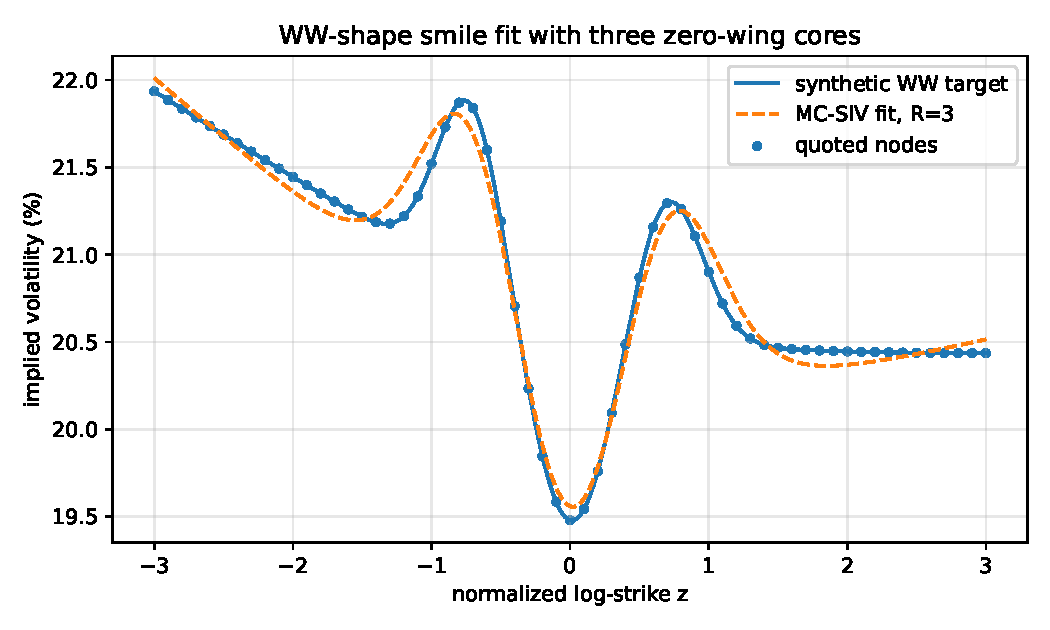
\includegraphics[width=0.82\textwidth]{mcsiv_figures/ww_fit.pdf}
\caption{Synthetic WW-shaped implied-volatility target and the three-core MC-SIV fit.  The fit uses a base log-cosh smile core, two positive zero-wing shoulder hats, and one negative zero-wing central notch.}
\label{fig:ww-fit}
\end{figure}

The volatility root-mean-square fitting error on the 61 nodes is
\begin{equation}
  \mathrm{RMSE}_\sigma=8.62\times10^{-4},
\end{equation}
that is approximately $8.6$ volatility basis points.  The maximum absolute node error is $2.14\times10^{-3}$, approximately $21.4$ volatility basis points.

The fitted local features are close to the target:
\begin{table}[t]
\centering
\caption{Interior WW features of target and MC-SIV fit.  Volatilities are annualized percentages.}
\label{tab:ww-features}
\begin{tabular}{@{}lcc@{}}
\toprule
Feature & Target $(z,\sigma)$ & MC-SIV fit $(z,\sigma)$ \\
\midrule
Left shoulder maximum & $(-0.77,\;21.88\%)$ & $(-0.84,\;21.81\%)$ \\
Central trough & $(0.01,\;19.48\%)$ & $(0.02,\;19.56\%)$ \\
Right shoulder maximum & $(0.73,\;21.30\%)$ & $(0.79,\;21.25\%)$ \\
\bottomrule
\end{tabular}
\end{table}

Figure \ref{fig:ww-components} shows the variance decomposition.  The shoulder hats and central notch are not special event objects; they are generic signed zero-wing SIV atoms.

\begin{figure}[t]
\centering
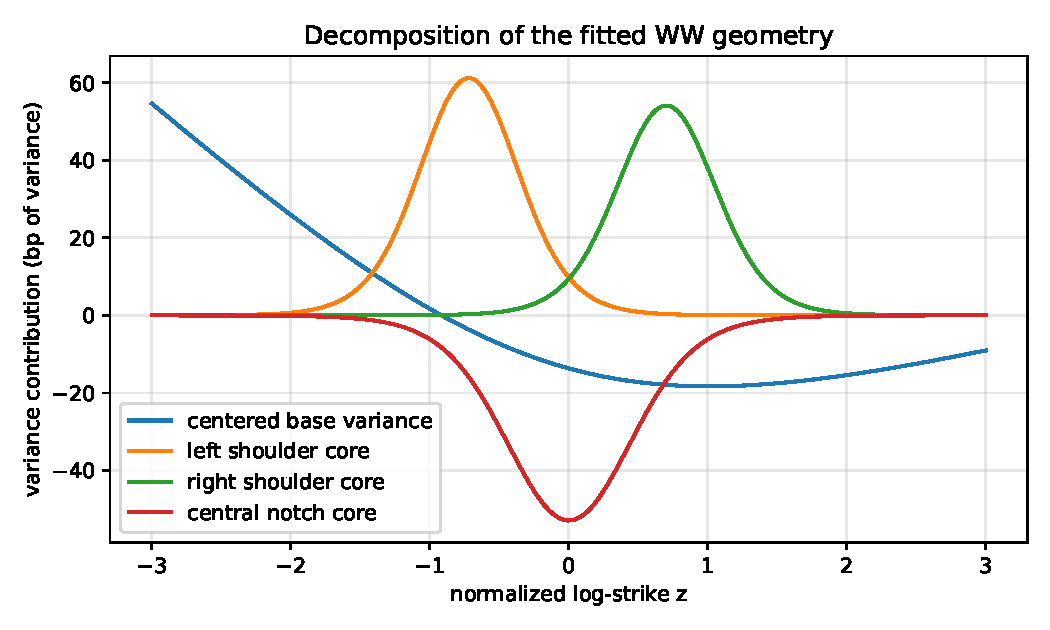
\includegraphics[width=0.82\textwidth]{mcsiv_figures/ww_components.pdf}
\caption{Component decomposition of the fitted WW geometry.  The base controls level, skew, and wings.  The two positive shoulder cores lift the left and right near-ATM regions; the negative central core creates the trough.}
\label{fig:ww-components}
\end{figure}

\subsection{No-arbitrage diagnostic for the example}

For the same fitted curve, take $T=7/365$ and $\sigref=20\%$.  On the grid $z\in[-5,5]$, the minimum fitted annualized variance is
\begin{equation}
  \min v_{\mathrm{fit}}(z)=0.03824,
\end{equation}
and the minimum Durrleman/Gatheral diagnostic is
\begin{equation}
  \min g(k)=0.1553.
\end{equation}
The right and left $z$-wing slopes of the illustrative linear-plus-log-cosh base are
\begin{equation}
  \lim_{z\to+\infty}v'(z)=0.000824,
  \qquad
  \lim_{z\to-\infty}v'(z)=-0.003131,
\end{equation}
so Lee's slope checks are far inside the bound for this short maturity.  Figure \ref{fig:g-diagnostic} shows the grid diagnostic.  This is not a proof that arbitrary amplitudes are arbitrage-free; it demonstrates the intended workflow: signed local cores are allowed, but they must be paired with explicit density checks.

\begin{figure}[t]
\centering
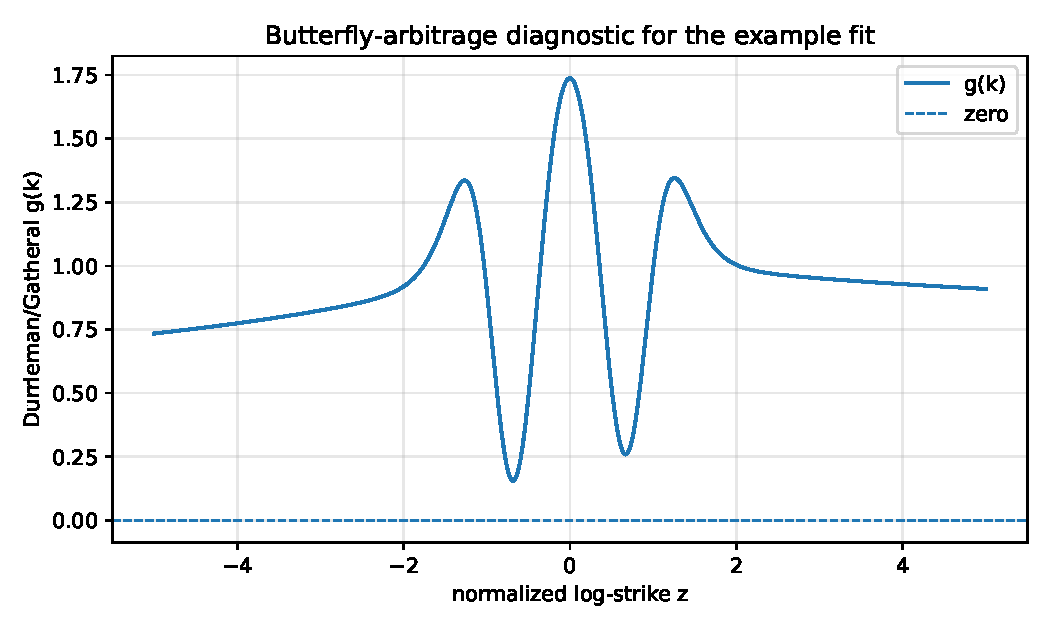
\includegraphics[width=0.82\textwidth]{mcsiv_figures/ww_g_diagnostic.pdf}
\caption{Butterfly-arbitrage diagnostic for the synthetic WW fit.  The plotted $g(k)$ is positive on the displayed grid.  Production calibration should enforce a positive margin and refine around local minima of $g$.}
\label{fig:g-diagnostic}
\end{figure}

\section{Calibration methodology}
\label{sec:calibration}

\subsection{Recommended objective}

The production objective should be price-space, not pure volatility-space, unless quotes are already cleaned and uniformly reliable.  A standard slice objective is
\begin{align}
  \min_{\theta,\psi}
  \quad
  \mathcal{L}(\theta,\psi)
  ={}&\sum_{i=1}^{N}\omega_i
  \left(
    C_{\mathrm{BS}}(F,K_i,T,w_i(\theta,\psi))-C_i^{\mathrm{mkt}}
  \right)^2
  \nonumber\\
  &+\lambda_1\sum_{r=1}^{R}|\alpha_r|
  +\lambda_2\sum_{r=1}^{R}\alpha_r^2
  +\lambda_{\mathrm{shape}}\,\mathcal{P}_{\mathrm{shape}},
  \label{eq:calibration-objective}
\end{align}
where
\begin{equation}
  w_i(\theta,\psi)=T\,v_R\!\left(\frac{\log(K_i/F)}{\sigref\sqrt{T}};\theta,\psi\right),
  \qquad
  \psi=\{(\alpha_r,c_r,h_r,\kappa_r)\}_{r=1}^{R}.
\end{equation}
The $\ell^1$ penalty encourages a sparse number of active hats, while the $\ell^2$ penalty stabilizes amplitudes when kernels overlap.

For fixed $(\theta,c_r,h_r,\kappa_r)$, the kernel amplitudes are linear in variance space.  If $y_i$ denotes target variance residual after the base fit and $X_{ir}=B_{c_r,h_r,\kappa_r}(z_i)$, the ridge estimate is
\begin{equation}
  \widehat{\alpha}
  =(X^\top W X+\lambda_2 I)^{-1}X^\top W y.
  \label{eq:linear-amplitude-fit}
\end{equation}
This conditional linearity is useful for initialization even when the final objective is price-space.

\subsection{Constraints and penalties}

The following constraints should be treated as hard constraints or high-weight barriers:
\begin{align}
  v_R(z_i)&\ge \eps_v,
  \label{eq:v-positive-grid}\\
  g(k_i)&\ge \eps_g,
  \label{eq:g-positive-grid}\\
  0&\le \frac{\sqrt{T}}{\sigref}W_C\le2-\eps_L,
  \qquad
  0\le \frac{\sqrt{T}}{\sigref}W_P\le2-\eps_L.
  \label{eq:lee-grid}
\end{align}
A smooth barrier for the density constraint is, for example,
\begin{equation}
  \mathcal{P}_{g}
  =\sum_i \softplus\!\left(\frac{\eps_g-g(k_i)}{\delta}\right)^2.
  \label{eq:g-barrier}
\end{equation}
After convergence, the minimum of $g$ should be refined between grid points by scalar minimization on intervals where $g$ is small.

Practical parameter bounds for local kernels are
\begin{equation}
  c_r\in[z_{\min}-\Delta,z_{\max}+\Delta],
  \qquad
  h_r\in[h_{\min},h_{\max}],
  \qquad
  \kappa_r\in[\kappa_{\min},\kappa_{\max}],
  \label{eq:kernel-bounds}
\end{equation}
with typical starting ranges
\begin{equation}
  h_{\min}\approx0.15,
  \quad
  h_{\max}\approx1.50,
  \quad
  \kappa_{\min}\approx1,
  \quad
  \kappa_{\max}\approx12.
\end{equation}
The exact values depend on quote density in $z$-space.  A sparse short-dated chain should not be allowed to fit extremely narrow kernels between quoted strikes.

\subsection{Robust fitting workflow}

A robust implementation can be organized as follows.
\begin{enumerate}[leftmargin=2em]
  \item Fit the base SIV slice with $R=0$ using the existing trader-parameter mapping.
  \item Compute residuals in price space and variance space.  Variance residuals are useful for shape diagnosis; price residuals drive the objective.
  \item Build a small dictionary of candidate hats over centers $c$, half-widths $h$, and steepnesses $\kappa$.
  \item Select one or more candidates by residual correlation, constrained least squares, or greedy reduction in the price objective.
  \item Fit amplitudes conditionally by a linear or ridge step.
  \item Refine $(\theta,\alpha,c,h,\kappa)$ jointly with bound constraints and no-arbitrage penalties.
  \item Prune kernels with small amplitudes or high overlap.  Refit after pruning.
  \item Repeat for $R=0,1,2,3$ and choose the smallest $R$ that passes quote-error and arbitrage tolerances.  A BIC-style criterion is often adequate:
  \begin{equation}
    \mathrm{BIC}_R=N\log(\mathrm{RSS}_R/N)+p_R\log N,
    \qquad p_R=6+4R.
  \end{equation}
\end{enumerate}
The rule should be conservative: use extra cores only when they materially reduce price residuals or remove a systematic WW residual.

\subsection{Identifiability safeguards}

Signed local kernels can be over-complete.  To reduce parameter degeneracy:
\begin{itemize}[leftmargin=2em]
  \item normalize all hats by \eqref{eq:B-def}, so amplitudes are in variance units;
  \item order centers, $c_1\le c_2\le\cdots\le c_R$, to remove label switching;
  \item impose a minimum center separation unless two kernels have clearly different scales;
  \item penalize overlapping kernels, for example through
  \begin{equation}
    \lambda_{\mathrm{overlap}}\sum_{r<s}
    \left(
      \frac{\langle B_r,B_s\rangle_W}
           {\|B_r\|_W\|B_s\|_W}
    \right)^2;
  \end{equation}
  \item keep $R\le3$ for ordinary listed-index smiles unless quote density justifies more.
\end{itemize}

\section{Minimal implementation skeleton}

The following code is intentionally minimal.  It shows the analytic kernel and the $g$ diagnostic; it omits option-price fitting, quote cleaning, and optimizer plumbing.

\begin{lstlisting}
import numpy as np


def safe_logcosh(x):
    x = np.asarray(x)
    return np.where(np.abs(x) < 50.0,
                    np.log(np.cosh(x)),
                    np.abs(x) - np.log(2.0))


def phi(u, kappa):
    return 4.0 / kappa**2 * safe_logcosh(0.5 * kappa * u)


def phi_p(u, kappa):
    return 2.0 / kappa * np.tanh(0.5 * kappa * u)


def phi_pp(u, kappa):
    return 1.0 / np.cosh(0.5 * kappa * u)**2


def hat_raw(z, c, h, kappa):
    u = z - c
    return phi(u - h, kappa) - 2.0 * phi(u, kappa) + phi(u + h, kappa)


def hat_raw_p(z, c, h, kappa):
    u = z - c
    return phi_p(u - h, kappa) - 2.0 * phi_p(u, kappa) + phi_p(u + h, kappa)


def hat_raw_pp(z, c, h, kappa):
    u = z - c
    return phi_pp(u - h, kappa) - 2.0 * phi_pp(u, kappa) + phi_pp(u + h, kappa)


def hat_norm_factor(h, kappa):
    return 2.0 * phi(h, kappa)


def hat(z, c, h, kappa):
    return hat_raw(z, c, h, kappa) / hat_norm_factor(h, kappa)


def hat_p(z, c, h, kappa):
    return hat_raw_p(z, c, h, kappa) / hat_norm_factor(h, kappa)


def hat_pp(z, c, h, kappa):
    return hat_raw_pp(z, c, h, kappa) / hat_norm_factor(h, kappa)


def add_multicores(z, base_v, base_vz, base_vzz, cores):
    # cores is a list of tuples (alpha, c, h, kappa).
    v = np.array(base_v, copy=True)
    vz = np.array(base_vz, copy=True)
    vzz = np.array(base_vzz, copy=True)
    for alpha, c, h, kappa in cores:
        v += alpha * hat(z, c, h, kappa)
        vz += alpha * hat_p(z, c, h, kappa)
        vzz += alpha * hat_pp(z, c, h, kappa)
    return v, vz, vzz


def gatheral_g_from_z(z, v, vz, vzz, T, sigma_ref):
    # k = sigma_ref * sqrt(T) * z, w = T * v.
    k = sigma_ref * np.sqrt(T) * z
    w = T * v
    wk = np.sqrt(T) / sigma_ref * vz
    wkk = vzz / sigma_ref**2
    return ((1.0 - k * wk / (2.0 * w))**2
            - 0.25 * wk**2 * (1.0 / w + 0.25)
            + 0.5 * wkk)
\end{lstlisting}

\section{Term structure without an event layer}

The generic surface form is
\begin{equation}
  w(k,T_n)
  =T_n\left[
    v_{\mathrm{SIV}}(z_n;\theta_n)
    +\sum_{r=1}^{R_n}\alpha_{n,r}B_{c_{n,r},h_{n,r},\kappa_{n,r}}(z_n)
  \right],
  \qquad
  z_n=\frac{k}{\sigref(T_n)\sqrt{T_n}}.
  \label{eq:surface-form}
\end{equation}
No additional event term is needed.  The surface problem is the standard one:
\begin{equation}
  \min \sum_{n,i}\omega_{n,i}\big(C_{n,i}^{\mathrm{model}}-C_{n,i}^{\mathrm{mkt}}\big)^2
  +\lambda_T\mathcal{R}_T
  +\lambda_K\mathcal{R}_K
  \label{eq:surface-objective}
\end{equation}
subject to slice positivity, butterfly constraints, Lee tail bounds, and calendar monotonicity.  A simple temporal roughness penalty is
\begin{equation}
  \mathcal{R}_T
  =\sum_n\|\theta_{n+1}-\theta_n\|_{M_\theta}^2
  +\sum_n\sum_r |\alpha_{n+1,r}-\alpha_{n,r}|^2,
  \label{eq:temporal-regularity}
\end{equation}
where matched kernels can be tracked by center and width.  If a macro announcement induces a WW shape only in one or two short expiries, the sparse model will simply select non-zero local kernels for those expiries.  That is an empirical outcome of the generic model, not a separate structural layer.

\section{Summary}

The generic multi-core SIV extension can be summarized as follows.
\begin{enumerate}[leftmargin=2em]
  \item Keep the original SIV base because it provides stable level, skew, convexity, minimum-variance, and wing-slope controls.
  \item Add only zero-wing local hats constructed from the original log-cosh primitive.
  \item Allow signed amplitudes; otherwise a multi-core model remains globally convex and cannot fit WW geometry.
  \item Preserve the SIV wing map automatically: local hats do not change $W_P$ or $W_C$.
  \item Enforce no-arbitrage through total-variance positivity, Lee slope bounds, and the Durrleman/Gatheral $g(k)$ density diagnostic.
  \item Fit the smallest number of local cores needed.  For a typical near-ATM WW smile, two shoulder hats plus one central notch are enough.
\end{enumerate}

Thus the final recommendation is not an event-specific SIV model, but a sparse generic multi-core SIV model:
\begin{equation}
  \boxed{
  v_R(z)=v_{\mathrm{SIV}}(z)+\sum_{r=1}^{R}\alpha_r B_{c_r,h_r,\kappa_r}(z),
  \qquad R\le3\text{ in ordinary use.}
  }
\end{equation}
This is flexible enough to fit WW-shaped curves while retaining the original SIV model's closed-form calculus and wing discipline.

\begin{thebibliography}{9}

\bibitem{sivdoc}
Model Documentation: Sigmoid-Implied Variance (SIV) Calibration.
Quantitative Research / Volatility Modeling, 29 March 2026.
User-provided internal note.

\bibitem{lee2004}
R. W. Lee.
\newblock The moment formula for implied volatility at extreme strikes.
\newblock \emph{Mathematical Finance}, 14(3):469--480, 2004.
\newblock \url{https://math.uchicago.edu/~rl/moment.pdf}

\bibitem{gatheraljacquier2014}
J. Gatheral and A. Jacquier.
\newblock Arbitrage-free SVI volatility surfaces.
\newblock \emph{Quantitative Finance}, 14(1):59--71, 2014.
\newblock \url{https://arxiv.org/abs/1204.0646}

\bibitem{roper2010}
M. Roper.
\newblock Arbitrage free implied volatility surfaces.
\newblock Working paper, University of Sydney, 2010.
\newblock \url{https://talus.maths.usyd.edu.au/u/pubs/publist/preprints/2010/roper-9.pdf}

\bibitem{alexiou2025}
L. Alexiou, A. Goyal, A. Kostakis, and L. Rompolis.
\newblock Pricing event risk: evidence from concave implied volatility curves.
\newblock \emph{Review of Finance}, 29(4):963--1007, 2025.
\newblock \url{https://academic.oup.com/rof/article/29/4/963/8079062}

\bibitem{baker2018}
M. Baker, T. Gillberg, and S. Thomas.
\newblock Trading events: smiles, frowns and moustaches -- the many faces of the options market.
\newblock SSRN working paper, 2018.
\newblock \url{https://papers.ssrn.com/sol3/papers.cfm?abstract_id=3263368}

\end{thebibliography}

\end{document}
